\documentclass{article}

\usepackage{amsmath, amssymb}
\usepackage{graphicx}

% cache of command for profiling:
% c:\anaconda3\python -m cProfile -s time hw_2015-12-16_v2.py -N 300 -L 5 0.1

\begin{document}
\title{MATH 441 Final Project}
\author{James Starkman, jas497}
\date{2015-12-16}
\maketitle

\vspace{-1em}


%% Write a paper of about 5 pages detailing your implementation and exploration
%% of the model; some of this will be a restatement of what is in the paper, but
%% you should also include any details that were left out of the original paper.

%% You should make sure to describe any ambiguities you resolved or differences
%% between your implementation and the implementation in the paper.

%% You should make sure to describe any features that you observe about the
%% model, i.e. the dynamics you observe over time and if you can get different
%% behavior from the model by changing a parameter value, etc.

%% It would be a good idea to include figures, plots, and frames of the
%% evolution of the model.

%% If you would like to, I would also be happy to see movies of the temporal
%% evolution.

%% Please organize the paper with an introduction describing why this problem is
%% important, a section describing the implementation of your model and any
%% observations, and a discussion where you summarize what you've done and
%% discuss any questions that the model could potentially resolve.

%%%%%%%%%%%%%%%%%%%%%%%%%%%%%%%%%%%%%%%%%%%%%%%%%%%%%%%%%%%%%%%%%%%%%%%%%%%%%%%%
%%%%%%%%%%%%%%%%%%%%%%%%%%%%%%%%%%%%%%%%%%%%%%%%%%%%%%%%%%%%%%%%%%%%%%%%%%%%%%%%
%%%%%%%%%%%%%%%%%%%%%%%%%%%%%%%%%%%%%%%%%%%%%%%%%%%%%%%%%%%%%%%%%%%%%%%%%%%%%%%%

\section{Introduction}

This problem is important because it provides us with a conceptually-simple
model of self-driven particles that nevertheless produces complex behavior.  For
example, consider a herd of large quadrupeds, such as buffalo, and suppose that
some external event startles them all (such as a loud noise coming from no
apparent direction), causing them all to charge in initially-random directions
at top speed (assumed constant) (assuming no collisions).  This model helps
determine how the herd as a whole moves, so their behavior can be predicted and
dealt with.  Specifically, since for small $\eta$ the flow usually converges
into a single direction, people who are in the path of the herd could be warned and 
take appropriate action, such as scaring the leaders into turning away.

\section{Implementation \&\ Observations} %%%%%%%%%%%%%%%%%%%%%%%%%%%%%%%%%%%%%%
\subsection{Implementation}

The model was implemented in Python 3.4 with the \verb|matplotlib| plotting
library (see the \verb|hw_2015-12-16_v2.py| file, included).  For values $N=300,
L=5, \eta=0.1$ (same as for figure 1d in the paper) and using the tile-based
version, each time step (also referred to as each ``tick'', ``update'',
``integration step'', \&c.; the meaning should be clear regardless of name,
however) took about 0.5--0.6 seconds to compute on a machine running Windows
10.1511, with a processor with a 6MB cache running at 2.4GHz.  The program
redrew (and made visible) the scatter plot each frame, producing the
visualisation live.  When the plots were disabled, it was substantially quicker,
taking closer to 150--200 milliseconds per tick.


The model has a command-line interface (uses the deprecated \verb|optparse|
module).  Details on running it are provided by executing it with the \verb|-h|
option at the system shell.


The code itself is mostly documented, and for the most part will not be
discussed here.


The algorithm for computing the local average angle is as follows.  First, the
sums of all of the x-components of the velocities (and same for y) of each
particle that lies within the radius of influence (semi-arbitrarily (and
certainly conveniently) set to unity) of the given particle were computed.  Then
the average angle is the arctangent of their ratio ($y$ over $x$, not vice
versa).  This matches what the model in the paper does, since

\begin{equation*}
  \begin{array}{rl}
    \arctan(\overline{\sin(\theta_i)} \div \overline{\cos(\theta_i)})
    &=
    \arctan((\frac{1}{N}\sum_{i=1}^N\sin(\theta_i)) \div (\frac{1}{N}\sum_{i=1}^N\cos(\theta_i)))\\
    &=
    \arctan((\sum_{i=1}^N\sin(\theta_i)) \div (\sum_{i=1}^N\cos(\theta_i)))\\
    &=
    \arctan((v\sum_{i=1}^N\sin(\theta_i)) \div (v\sum_{i=1}^N\cos(\theta_i)))\\
    &=
    \arctan((\sum_{i=1}^N v\sin(\theta_i)) \div (\sum_{i=1}^N v\cos(\theta_i)))
  \end{array}
\end{equation*}

\noindent
and $v\sin(\theta)$ is the y-component of the particles velocity (and
$v\cos(\theta)$ is the x-component).  The resulting average angle can then be
perturbed, and the new angle used to make the new velocity.  These
implementations both then use this new velocity to compute the new position, and
leave the new velocity where the next iteration can find it.


A time step of 1 was used, to make the paper's value of $v=0.03$ make sense and
to save multiplication.


$v_a$ is defined to have ``converged'' if the standard deviation of the last ten
values (including the current value) is less than a cutoff of 0.01, and if there
have been more than ten ticks.  The former condition is based on empirical
observation of the values for $v_a$ (which can be printed to stdout each tick
with \verb|-v|), while the latter ensures that there always will be ten elements
of which to compute the standard deviation.  In addition, in order to force the
more chaotic systems to converge, the cutoff for the standard deviation was
increased by 0.01 every five hundred ticks.  These numbers were determined
experimentally based on what looked about right.

\subsection{Observations} %%%%%%%%%%%%%%%%%%%%%%%%%%%%%%%%%%%%%%%%%%%%%%%%%%%%%%

\subsubsection{Recreating figure 1 from the paper}

Execution: this looks best with the \verb|-pfv| options enabled.

The model behaves as described in the paper.  For compatibility with the paper,
all figures in this sub-subsection used $N=300$.  They were simulated with both
the \verb|-p| and the \verb|-f| options, and \verb|^C| when finished.


As a baseline, of sorts, a run was done with $\eta=2\pi$, to obtain complete
anarchy.  This goal was realized: $v_a$ almost never went above 0.1, and the
motion looked like the animations of gas particles that one sees in physics
classes, but without the collisions.  A figure is not included because there is
nothing interesting in random scatter.


See figure \ref{fig:state_lowrho} for evolution of a low-density, low-randomness
simulation (like figure 1b in the paper).  These show how clumps form and
migrate, travelling close to the theoretical limit of 0.03 distance units per
tick (which is only achieved if \emph{all} particles travel in the \emph{exact}
same direction, thus never being observed (although if one sets $\eta=0$, one
can get more than six nines after the decimal point after fairly few ticks)).

\begin{figure}[ht]
  \centering 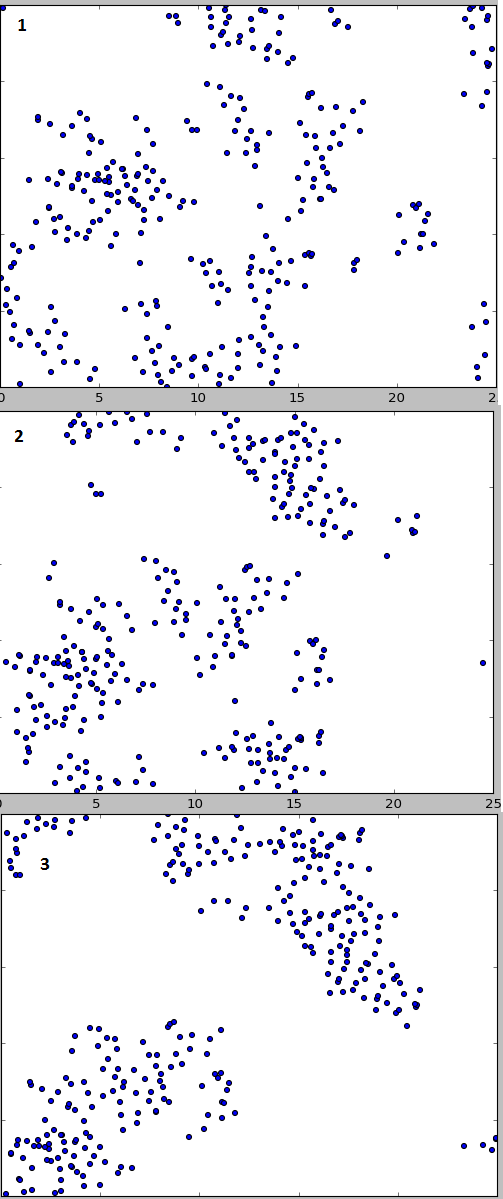
\includegraphics[height=7in]{2015-12-16_state_lowrho.png}
  \caption{\label{fig:state_lowrho} $L=25, \eta=0.1$.  States in figure were
    captured after one, two, and three minutes of runtime, respectively (model
    ran at almost exactly three ticks per second).  At time of the third image,
    $v_a=0.84$.}
\end{figure}

For the recreation of figure 1c in the paper, the particles quickly became
ordered, and all drifted in about the same direction early on in the model,
although they did not form tight currents, only general tides.  Upping $\eta$ to
3.14 (thus allowing up to a sudden right turn due to randomness) better
recreated the result, with $v_a\in[0.5,0.6]$ being mostly true for ticks
\#12--200.  Regarding movements (which cannot really be shown in a figure), the
particles started by juddering about the same places that they were created, but
eventually aligned into a sluggish stream.  Each individual frame still looked
like scatter, however.


For the recreation of figure 1d in the paper, the particles became ordered
\emph{very} rapidly, reaching $v_a>0.999$ in under twenty ticks (according to
one run).  However, even after several minutes of simulation (tick \#400), they
still did not meld into coherent streams like the figure in the paper, and
instead stayed as sparse as they were at the beginning.  Each individual frame
looked like scatter, so a figure would not show it properly and thus is not
included.

\subsubsection{Recreating figure 2 from the paper}

Execution: this sub-subsection uses the \verb|-s| option.  Neither of the
options \verb|-pf| are recommended to use in combination with this, and one
should probably not use \verb|-v|, either (although there is no harm in it).


To produce the plots in figures \ref{fig:summary_eta} and \ref{fig:summary_rho},
three runs were done under the same conditions, and their resulting $v_a$ values
averaged.  This is why they look jagged, but less jagged than they might
otherwise be.


Regarding figure \ref{fig:summary_eta}, it is observed that, as $\eta$
increased, more time steps were required for convergence.  Without the increases
in the tolerance of the standard deviation every five hundred ticks, this would
have taken much longer (full disclosure: the version of the code with the
tolerance was started about an hour after the flat 0.01 version, and finished in
an hour.  The other process, which was still running, was then killed, so its
total runtime is unknown.  However, it regularly took many thousands of ticks to
converge, so the tolerance cutoff increase certainly makes a difference for
runtime).  As can be seen, the plot looks similar to the one in the paper ---
low $\eta$ implies high $v_a$ and vice versa.  More simulation runs per value of
$\eta$ would make this appearance more clear, as well as reduce the jitter for
low $\eta$.


Regarding figure \ref{fig:summary_rho}, it is observed that, when $\rho=0.1$,
each tick took about 10ms to compute; larger values for $\rho$ mean more
particles, so this can be seen as a compute-time ``lower bound'', of sorts.
Note that the figure in the paper is for an unspecified value of $\eta$, which
has been assumed to be 0.1 for the recreation.  For comparison, when a value of
$\eta=\frac{3\pi}{4}$ was used, the plot looked like line noise, as when
$\eta=0.5$.  Here, although it still looks like line noise, now a trend can be
seen.  $v_a$ is never large for small densities, and never truly small for large
$\rho$ (note: initially, when all velocity directions are uniformly random,
$v_a$ is usually less that 0.05 (and after running with $\eta=2\pi$, less than
0.1), so anything much above that indicates \emph{some} level of order).

\begin{figure}[ht]
  \centering 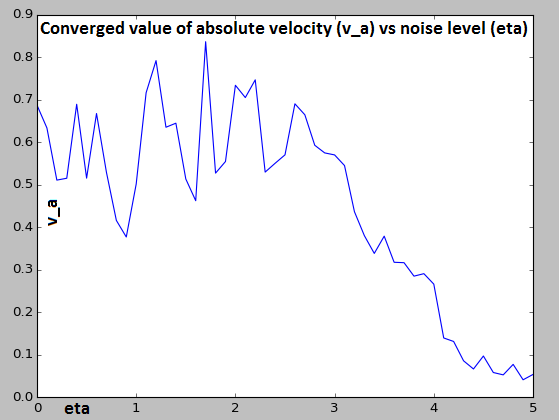
\includegraphics[width=\textwidth]{2015-12-16_summary_eta.png}
  \caption{\label{fig:summary_eta} $N = 400, L = 10$.  This took about 63
    minutes to produce.}
\end{figure}

\begin{figure}[ht]
  \centering 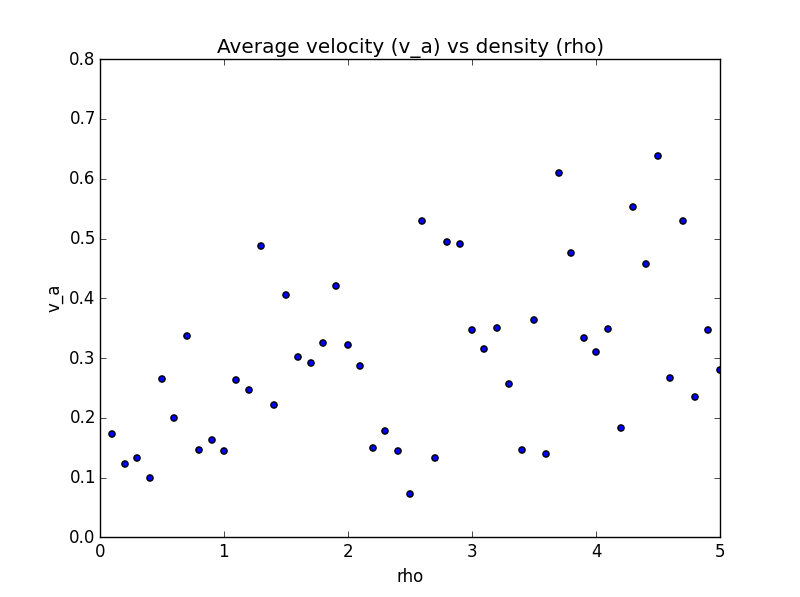
\includegraphics[width=\textwidth]{2015-12-16_summary_rho.png}
  \caption{\label{fig:summary_rho} $L = 20, \eta = 0.1$.  This took about 23
    minutes to produce.}
\end{figure}


\section{Discussion} %%%%%%%%%%%%%%%%%%%%%%%%%%%%%%%%%%%%%%%%%%%%%%%%%%%%%%%%%%%

The meanings of the observations are inlined, and are not repeated here in full.
However, to summarize, it was found that this implementation of the model mostly
matches the behavior of the model in the paper, with the differences probably
due to the stochastic nature of the model.  Also, there were a few parameters
missing from the paper whose values cannot be easily divined, so the differences
could also be due to that.  Visually, watching the model evolve reveals that it
functions about as expected, in particular with regard to the formation of small
herds that move on their own (see figure \ref{fig:state_lowrho}).

\end{document}
